% --------------------------------
\chapter{Análisis de resultados}
% --------------------------------
\label{C:sobre_LaTeX}
En esta sección se comprobó el funcionamiento completo de la aplicación diseñada por medio de un estudio de caso, en el que se tomó la placa de un activo para poder realizar el proceso completo de registro. A partir de ello se discutió los resultados obtenidos y se mostró cuales posibles escenarios alternativos podría presentar en su funcionamiento.
\par

\section{Estudio de caso}
Para este estudio de caso se tomó la placa de una silla de la sala de estudio (que previamente se registró en las pruebas), una placa de un monitor sin registrar y una foto sin ninguna placa en ella. Se inició colocando la placa de la silla de la sala de estudio dentro del rango de la cámara, cómo se puede apreciar en la figura \ref{r:uno}. Este es el primer paso necesario para el registro, es importante destacar, que debido al proceso de entrenamiento que se aplicó a la red neuronal y a los parámetros de preprocesado de imágenes utilizado, los resultados pueden ser obtenidos aún cuando la imagen no sea lo más clara o no esté lo suficientemente centrada. 

\begin{figure}[ht]
    \centering
    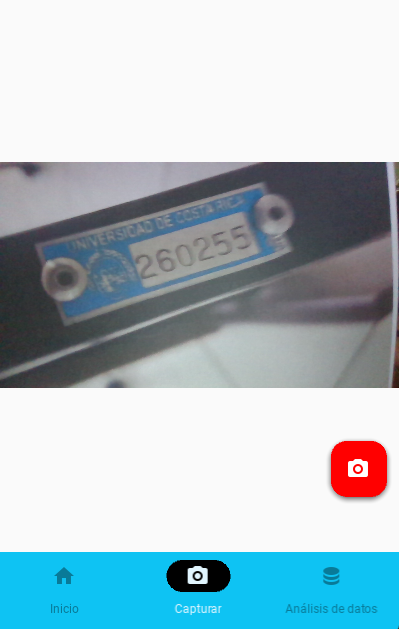
\includegraphics[width=0.35\textwidth]{imagenes/resultados/uno.png}
    \caption{Paso uno del registro de placas}
    \label{r:uno}
\end{figure}
\par
Una vez que se determinó que la imagen se encontraba apta para que la red la procese, se oprime el botón rojo de captura, lo cual en caso de ser correcto muestra una notificación en pantalla como se puede observar en la figura \ref{r:dos}, por lo que el usuario se notifica de la posibilidad de avanzar al análisis de datos.
\begin{figure}[ht]
    \centering
    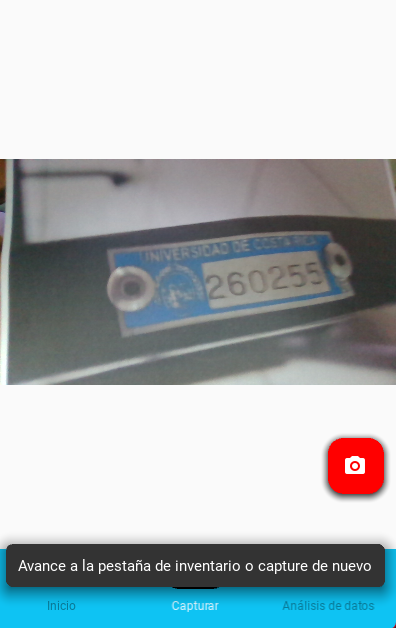
\includegraphics[width=0.35\textwidth]{imagenes/resultados/dos.png}
    \caption{Paso dos del registro de placas}
    \label{r:dos}
\end{figure}
\par
Cuando se oprime el botón de análisis de datos, se accede a la BD y se despliega la información de la placa, en este caso se escaneó una placa previamente registrada, por lo que los datos anteriores también se presentan en el espacio lleno para que se puedan ver y modificar, así como se ve en la figura \ref{r:tres}.
\begin{figure}[ht]
    \centering
    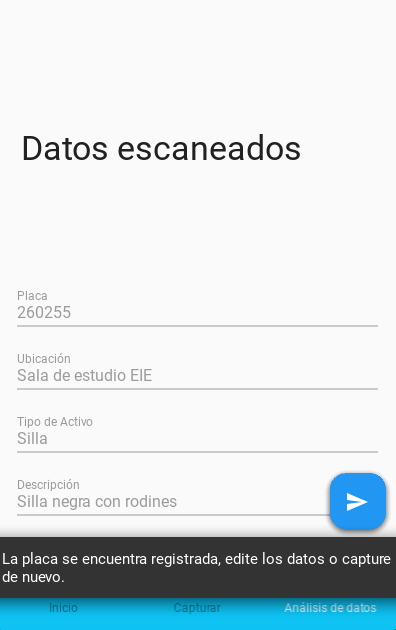
\includegraphics[width=0.35\textwidth]{imagenes/resultados/tres.png}
    \caption{Paso tres del registro de placas}
    \label{r:tres}
\end{figure}
\par
El usuario deberá modificar los valores que así lo requieran y una vez se decide que la información está completa, únicamente se oprime el botón de enviar y cuando se completa la solicitud a la BD, la aplicación despliega un mensaje como en la figura \ref{r:cuatro}. Con esto se completa un proceso de registro (en este caso modificación) de un activo de la EIE. 
\begin{figure}[ht]
    \centering
    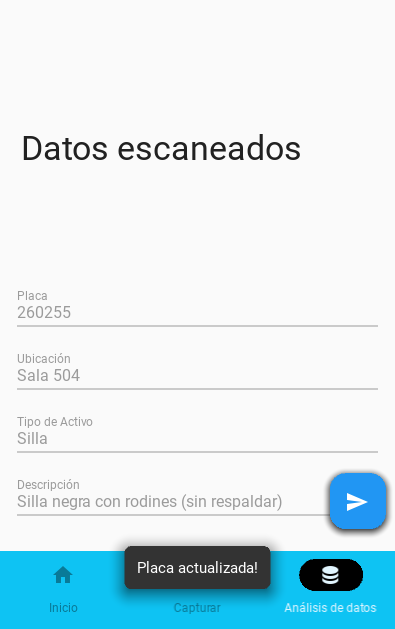
\includegraphics[width=0.35\textwidth]{imagenes/resultados/cuatro.png}
    \caption{Último paso del registro de placas}
    \label{r:cuatro}
\end{figure}
\par
El registro puede presentar variaciones dependiendo de lo que se requiere hacer, cuando una placa no se encuentra en la base de datos, únicamente el espacio de placa se llena por el usuario para que pueda añadir los valores de la misma como en la figura \ref{r:cinco}. Una vez registrada el mensaje que despliega la aplicación al usuario es la de registro exitoso en vez de que se actualizó la placa. Otro caso es cuando la imagen es ilegible por la red neuronal, aquí se avisa al usuario desde la misma pantalla de captura, que no es posible identificar la placa y que debe retomar la captura, de forma equivalente a la figura \ref{r:seis}.
\begin{figure}[ht]
    \centering
    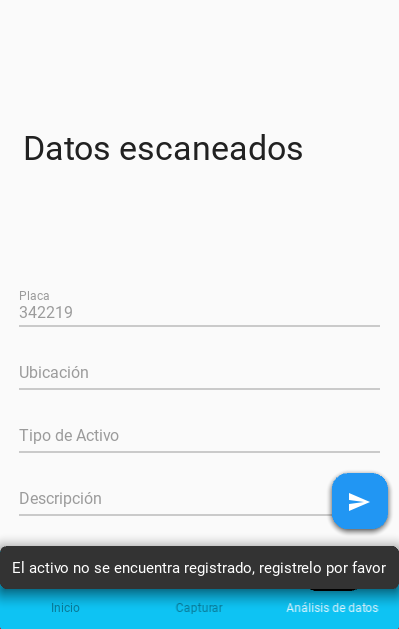
\includegraphics[width=0.35\textwidth]{imagenes/resultados/cinco.png}
    \caption{Comportamiento de la aplicación ante un registro de una nueva placa.}
    \label{r:cinco}
\end{figure}
\begin{figure}[ht]
    \centering
    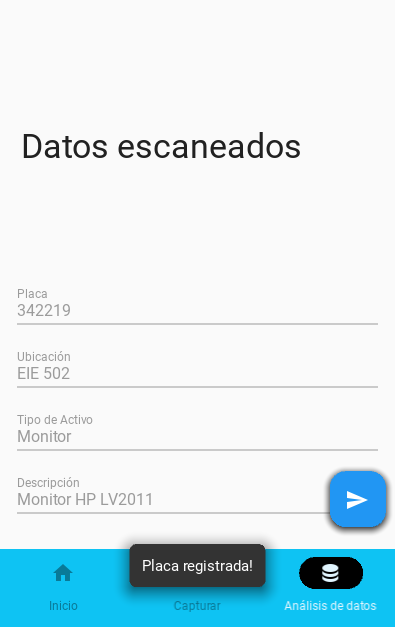
\includegraphics[width=0.35\textwidth]{imagenes/resultados/seis.png}
    \caption{Comportamiento de la aplicación ante una captura ilegible para la red neuronal.}
    \label{r:seis}
\end{figure}